%%%%%%%%%%%%%%%%%%%%%%%%%%%%%%%%%%%%%%%%%%%%%%%%%%%%%%%%%%%%%%%%%%%%%%%%%%%%%%
% COMP 9200 Assignment 3, Part 1 -- AI-assisted vs. own analysis (pairs)
% Dataset: succinctly/midjourney-prompts (Hugging Face)
%
% Build:   latexmk -pdf COMP9200_A3_Part1_Paper.tex
% Numbers: every \Macro in the text comes from tables/numbers.tex, which
%          analysis/pipeline.py writes. Re-run the pipeline, rebuild, done.
% Status:  sections marked \todo{} still need writing. The methodology and
%          "our pipeline" results are drafted from the real pipeline output;
%          everything about the AI arm waits for the runs in ai-analysis/.
% Length:  4-6 pages. Check whether the appendix counts toward the limit.
%%%%%%%%%%%%%%%%%%%%%%%%%%%%%%%%%%%%%%%%%%%%%%%%%%%%%%%%%%%%%%%%%%%%%%%%%%%%%%

\documentclass[conference]{IEEEtran}
\IEEEoverridecommandlockouts

\usepackage{cite}
\usepackage{amsmath,amssymb,amsfonts}
\usepackage{graphicx}
\usepackage{textcomp}
\usepackage{xcolor}
\usepackage{booktabs}
\usepackage{array}
\usepackage[hidelinks]{hyperref}
\usepackage{url}

\newcommand{\todo}[1]{\textcolor{red}{[TODO: #1]}}
% Generated by analysis/pipeline.py -- do not edit by hand.
\newcommand{\NRaw}{246,381}
\newcommand{\NCorpus}{57,670}
\newcommand{\NDupRows}{180,983}
\newcommand{\PctDupRows}{73.5}
\newcommand{\PctNonPrompt}{51.2}
\newcommand{\PctTestLeak}{83.2}
\newcommand{\PctTestPromptLeak}{68.4}
\newcommand{\MedianChars}{15}
\newcommand{\MedianWords}{12}
\newcommand{\IQRWords}{7--21}
\newcommand{\PctAnyParam}{47.6}
\newcommand{\PctAspect}{36.1}
\newcommand{\PctWeight}{8.3}
\newcommand{\PctArtistStrict}{14.4}
\newcommand{\PctArtistLenient}{24.3}
\newcommand{\PctBoosterAny}{36.2}
\newcommand{\TopicJaccard}{0.81}
\newcommand{\HOneRankBiserial}{0.40}
\newcommand{\HTwoCramersV}{0.08}
\newcommand{\NPromptRows}{120,357}
\newcommand{\PctPromptRows}{48.8}
\newcommand{\ArtistRuleRatio}{1.7}
\newcommand{\NBoosters}{27}
\newcommand{\MedianWordsParam}{17}
\newcommand{\MedianWordsNoParam}{9}
\newcommand{\HTwoChi}{347.5}
\newcommand{\PctBoostIfArtist}{42.8}
\newcommand{\PctBoostIfNoArtist}{34.1}
\newcommand{\MinTopicJaccard}{0.52}


\title{Same Data, Two Analysts: Comparing Generative AI Tools with a
Scripted Pipeline on Midjourney Prompts}

% Shared affiliation stated once, above the names.
\author{
\IEEEauthorblockA{\textit{COMP 9200: Applied Research Methods} \\
\textit{British Columbia Institute of Technology}\\
Burnaby, Canada}
\\[0.6\baselineskip]
\begin{tabular}{@{}c@{\hspace{3em}}c@{\hspace{3em}}c@{}}
\large Christopher Elliott & \large Mitchell Winter & \large Boris Kim \\
\small celliott64@my.bcit.ca & \small mwinter18@my.bcit.ca &
\small skim743@my.bcit.ca
\end{tabular}
}

\begin{document}
\maketitle

\begin{abstract}
This study analyses \NRaw{} rows of user prompts from the Midjourney Discord server
with two generative AI tools (GitHub Copilot and Claude Code), each given
only the data and a fixed sequence of questions, and with a scripted Python
pipeline written by the authors. \PctNonPrompt\% of rows are not prompts, \PctDupRows\% are
exact duplicates, and \PctTestInTrain\% of test rows also appear in the
training split. For the \NCleanPrompts{} clean prompts, the paper reports prompt structure,
artist references, quality-booster phrases and topics. The AI
tools found the same data problems, used effect sizes and avoided causal
claims, but differed from the scripted pipeline wherever a definition had to be
chosen: what
counts as a prompt, how length is counted, and which artists and phrases are
searched for. On one hypothesis this turned a negligible effect into a
21-point difference. An AI analyst is one more analyst with its own hidden
choices, and its definitions need the same scrutiny as its numbers.
\end{abstract}

\begin{IEEEkeywords}
generative AI, data analysis, reproducibility, text-to-image prompts,
data quality, topic modelling
\end{IEEEkeywords}

%%%%%%%%%%%%%%%%%%%%%%%%%%%%%%%%%%%%%%%%%%%%%%%%%%%%%%%%%%%%%%%%%%%%%%%%%%%%%%
\section{Introduction}
%%%%%%%%%%%%%%%%%%%%%%%%%%%%%%%%%%%%%%%%%%%%%%%%%%%%%%%%%%%%%%%%%%%%%%%%%%%%%%

Generative AI tools can now load a data file, write and run analysis code,
and summarise the results in plain language. This makes them attractive as
research assistants, but it raises questions about rigor, transparency and
reproducibility: the analyst may not see the decisions the tool made, and
the same request can give different answers on different days.

This study gives the same public dataset and the same research questions
to two generative AI tools and to a scripted pipeline, and compares the
results. The dataset is a collection of text-to-image prompts
from the Midjourney Discord server \cite{succinctlyMidjourneyPrompts2022}.
It suits the comparison because it has a single free-text column, so every
variable has to be derived by rules the analyst chooses.

The research questions are:
\begin{itemize}
  \item \textbf{RQ1:} What does a typical prompt look like (length,
        parameters, aspect ratios)?
  \item \textbf{RQ2:} How often do prompts name an artist or use generic
        ``quality booster'' phrases?
  \item \textbf{RQ3:} What themes do prompts cover, and how stable are the
        topics found?
  \item \textbf{RQ4:} Are parameter use and prompt length related, and are
        artist references and booster phrases related?
\end{itemize}
For each question, the AI tools and the scripted pipeline are compared on
findings, rigor, transparency, bias and reproducibility.

%%%%%%%%%%%%%%%%%%%%%%%%%%%%%%%%%%%%%%%%%%%%%%%%%%%%%%%%%%%%%%%%%%%%%%%%%%%%%%
\section{Related Work}
%%%%%%%%%%%%%%%%%%%%%%%%%%%%%%%%%%%%%%%%%%%%%%%%%%%%%%%%%%%%%%%%%%%%%%%%%%%%%%

\textit{Text-to-image prompts.} Liu and Chilton derived design guidelines
for prompting text-to-image models \cite{liuDesignGuidelinesPrompt2022},
and Oppenlaender proposed a taxonomy of prompt modifiers such as style and
quality boosters \cite{oppenlaenderTaxonomyPromptModifiers2023}. Large
prompt collections such as DiffusionDB \cite{wangDiffusionDB2023} and
prompt-log studies \cite{xiePromptLogAnalysis2023} describe how users write
prompts in practice. % VERIFY both sentences below against the papers.
Both describe prompts as lists of subject and style keywords with frequent
reuse of the same modifiers, which RQ1 and RQ2 measure directly.

\textit{AI as data analyst.} Cheng et al.\ evaluated GPT-4 as a data
analyst \cite{chengGPT4GoodData2023} and found its output comparable to
human analysts on several criteria, but with errors in data handling and
reasoning that a reader could not see without checking the work.

\textit{Analytic flexibility and data quality.} Silberzahn et al.\ showed
that independent analysts given the same data reach different conclusions
\cite{silberzahnManyAnalysts2018}; an AI tool is one more analyst whose
choices may be hidden. Duplicates in text corpora inflate evaluation
results \cite{leeDeduplicating2022}, and datasheets
\cite{gebruDatasheets2021} were proposed to document how a dataset was
collected and what it should be used for.

%%%%%%%%%%%%%%%%%%%%%%%%%%%%%%%%%%%%%%%%%%%%%%%%%%%%%%%%%%%%%%%%%%%%%%%%%%%%%%
\section{Methodology}
%%%%%%%%%%%%%%%%%%%%%%%%%%%%%%%%%%%%%%%%%%%%%%%%%%%%%%%%%%%%%%%%%%%%%%%%%%%%%%

\subsection{Dataset}
\texttt{succinctly/midjourney-prompts} \cite{succinctlyMidjourneyPrompts2022}
contains \NRaw{} rows with a single \texttt{text} column, split into train
(221,743), validation (12,318) and test (12,320). It was derived from a
Kaggle scrape of the public Midjourney Discord server
\cite{kaggleMidjourney250k}, keeping only the user's text. It has no user
identifiers, timestamps or images, and is released under Apache-2.0. The Parquet files were downloaded on 6 Nov.\ 2026 and their SHA-256 hashes
recorded (Appendix~\ref{app:repro}).

\subsection{Preprocessing}
All rules are defined in one file (\texttt{prompt\_utils.py}) so they can be
quoted and checked.
\begin{itemize}
  \item \textit{Parameters} are tokens of the form \texttt{--name value}.
        Because phones and Discord often turn \texttt{--} into an en or em
        dash, all three are accepted. Names are mapped to canonical forms
        (e.g.\ \texttt{--ar} and \texttt{--aspect} to \textit{aspect}).
  \item \textit{Content words} are the alphabetic tokens left after
        removing parameters, URLs and \texttt{::} weights.
  \item \textit{Row type.} A row is a \textit{prompt} if it has at least
        three content words; otherwise it is classed as empty, aspect ratio
        only, number only, URL or parameters only, symbols only, or a short
        fragment (Table~\ref{tab:fragments}).
  \item \textit{Duplicates} are found after lower-casing and collapsing
        whitespace. The first copy is kept.
\end{itemize}
Because the provided splits overlap (Section~\ref{sec:quality}), the splits are pooled and repeated prompts removed, leaving \NCleanPrompts{} clean prompts
(Table~\ref{tab:flow}).

\begin{table}[t]
\centering
\caption{Row types in the raw data (all splits).}
\label{tab:fragments}
\begin{tabular}{lrr}
\toprule
Row type & Rows & \% \\
\midrule
prompt & 120,357 & 48.8 \\
short fragment & 59,726 & 24.2 \\
aspect ratio only & 34,571 & 14.0 \\
url or params only & 14,832 & 6.0 \\
number only & 13,922 & 5.7 \\
empty & 1,597 & 0.6 \\
symbols only & 1,376 & 0.6 \\
\bottomrule
\end{tabular}

\end{table}

\begin{table}[t]
\centering
\caption{From raw rows to clean prompts.}
\label{tab:flow}
\begin{tabular}{lr}
\toprule
Step & Rows \\
\midrule
Raw rows (all splits) & 246,381 \\
\quad excluded: not a prompt & 126,024 \\
Prompt rows & 120,357 \\
\quad excluded: duplicate & 62,687 \\
Analytic corpus & 57,670 \\
\bottomrule
\end{tabular}

\end{table}

\subsection{AI Tool Setup}
\textit{Run A} (8 Nov.\ 2026) used the GitHub Copilot agent in Visual
Studio Code; the chat export records the model only as
\texttt{gpt-6.1-terra}, with no published version. \textit{Run B} (11 Nov.\
2026) used the Claude Code extension with \texttt{claude-opus-5-5} at medium
effort. Run B is a second analyst, not a repeat of run A, and since a Claude model also helped write the scripted pipeline, it is the
less independent AI arm.
Each run started a fresh session with memory, custom instructions and web
search off (by the operator's account; the exports do not record this). The
tool worked in a local folder holding one file,
\texttt{midjourney\_prompts\_all.csv} (columns \texttt{split} and
\texttt{text}, \NRaw{} rows), ran its own Python code, and was not given the pipeline's rules or results. It received seven fixed prompts (P0--P6): an
open-ended request, one per research question, and a request for the
complete code (Appendix~\ref{app:prompts}), with no hints in between. Each
response was saved unedited and scored against the pipeline's results on findings,
rigor, transparency, bias and reproducibility.

\subsection{Scripted Pipeline}
The pipeline is a Python script (\texttt{pipeline.py}) using pandas, SciPy
and scikit-learn \cite{pedregosaScikitlearn2011}, with pinned library
versions and a fixed random seed. It checks the input files' hashes,
applies the preprocessing above, and writes every reported number, table
and figure, so the paper cannot drift from the code.

\textit{RQ1} reports medians and interquartile ranges of content words,
the share of prompts using each parameter, and aspect-ratio counts.

\textit{RQ2} detects artist references with two rules, to show how much the
answer depends on the rule: a \textit{strict} rule (``by'' or ``in the
style of'' followed by capitalised words) and a \textit{lenient} rule (the
same cue words in any case, split on ``and'' and commas). Quality boosters
are matched against a fixed list of \NBoosters{} phrases taken from common prompt
advice (e.g.\ ``trending on artstation'', ``8k'', ``octane render'').

\textit{RQ3} fits a TF-IDF representation (minimum document frequency 20,
English stop words removed) and non-negative matrix factorisation (NMF)
\cite{leeSeungNMF1999} with $k=10$ topics. To test stability, the model is refitted on five random 80\% subsamples,
each started from the same SVD-based initialisation as the reference model
(NNDSVDar); topics are matched to the reference run, and the Jaccard
overlap $J$ of their top ten words is reported.
% NOTE: this tests sensitivity to the sample only. On the full data,
% changing the seed with NNDSVDar gives J = 1.00 every time. With a fully
% random start (init="random") mean J drops from 0.81 to about 0.62.
% Decide whether to report that as well; see the comment in pipeline.py rq3().

\textit{RQ4} tests H1 (prompts with any parameter are longer) with a
Mann--Whitney $U$ test and rank-biserial correlation, and H2 (artist
references, under the lenient rule, are associated with booster phrases)
with a $\chi^2$ test and Cram\'er's $V$. With $n=\NCleanPrompts$, almost any difference is
significant, so effect sizes, not $p$-values, are interpreted.

%%%%%%%%%%%%%%%%%%%%%%%%%%%%%%%%%%%%%%%%%%%%%%%%%%%%%%%%%%%%%%%%%%%%%%%%%%%%%%
\section{Results}
%%%%%%%%%%%%%%%%%%%%%%%%%%%%%%%%%%%%%%%%%%%%%%%%%%%%%%%%%%%%%%%%%%%%%%%%%%%%%%

Table~\ref{tab:compare} sets the headline numbers side by side. The subsections give the scripted pipeline's results and then the AI
tools'.

\begin{table*}[t]
\centering
\caption{Headline results: AI tools (runs A and B) vs.\ the scripted pipeline.}
\label{tab:compare}
\small
\begin{tabular}{lllll}
\toprule
Question & Measure & Run A (Copilot) & Run B (Claude) & Scripted pipeline \\
\midrule
Data quality & Exact duplicate rows & 180,983 (73.5\%) & 180,983 (73.5\%) & \NDupRows{} (\PctDupRows\%) \\
             & Test rows also in train & 83.1\% & 83.1\% & \PctTestInTrain\% \\
             & Rows analysed after cleaning & 64,907 & 59,733 & \NCleanPrompts \\
RQ1 & Median length (IQR) & 12 (6--21)$^a$ & 12 (7--20) & \MedianWords{} (\IQRWords) \\
    & Any parameter & 42.2\% & 46.2\% & \PctAnyParam\% \\
    & \texttt{--ar}/\texttt{--aspect} & 31.8\% & 35.3\% & \PctAspect\% \\
RQ2 & Names an artist & 13.5\% (50 names) & 21.3\% (168 names) & \PctArtistStrict\% strict, \PctArtistLenient\% lenient \\
    & Booster phrase & 21.8\% (6 phrases) & 33.1\% (16 phrases) & \PctBoosterAny\% (\NBoosters{} phrases) \\
RQ3 & Topic stability & cosine 0.88, 0.76 & $J = 0.75$ (subsamples) & $J = \TopicJaccard$ (subsamples) \\
RQ4 & H1 effect size & $r_{rb} = 0.60$ & $r_{rb} = 0.41$ & $r_{rb} = \HOneRankBiserial$ \\
    & H2 effect size & OR $= 2.84$ ($V = 0.17$)$^b$ & OR $= 2.17$ ($V = 0.16$)$^c$ & $V = \HTwoCramersV$ \\
\bottomrule
\end{tabular}

\smallskip
\footnotesize $^a$Whitespace items, counting parameter flags and values as words; run B and the scripted pipeline count content words only.
$^b$The tool reported the odds ratio; $V$ is computed from the tool's $\chi^2$ and $n$.
$^c$Falls to OR $\approx 1.0$ when prompt length is controlled.
\end{table*}

\subsection{Data Quality}
\label{sec:quality}
Only \NPromptRows{} of \NRaw{} rows (\PctPromptRows\%) are prompts. The rest are bare
aspect ratios such as \texttt{16:9}, numbers, lone parameters such as
\texttt{--uplight}, and one- or two-word fragments
(Table~\ref{tab:fragments}). The median raw row is \MedianChars{}
characters long. \NDupRows{} rows (\PctDupRows\%) are exact duplicates of
an earlier row, and \PctTestInTrain\% of test rows (\PctTestPromptsInTrain\% of
test rows that are real prompts) also appear in train. A model trained and
evaluated on these splits would be tested largely on data it had already
seen \cite{leeDeduplicating2022}.

\subsection{RQ1: Prompt Structure}
Clean prompts have a median of \MedianWords{} content words (IQR
\IQRWords), with a long right tail (Fig.~\ref{fig:length}).
\PctAnyParam\% use at least one parameter; aspect ratio is by far the most
common (\PctAspect\%), led by 16:9 and 9:16 (Fig.~\ref{fig:params}).
\PctWeight\% use \texttt{::} weights. Most prompts are comma-separated
lists of descriptors rather than sentences.

\begin{figure}[t]
\centering
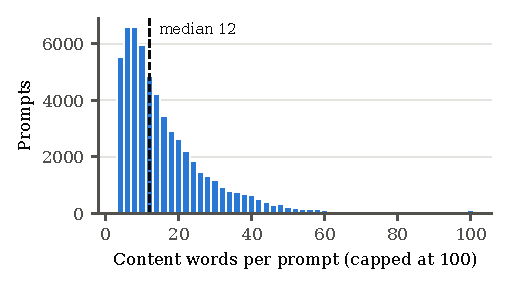
\includegraphics[width=\columnwidth]{figures/length}
\caption{Content words per clean prompt.}
\label{fig:length}
\end{figure}

\begin{figure}[t]
\centering
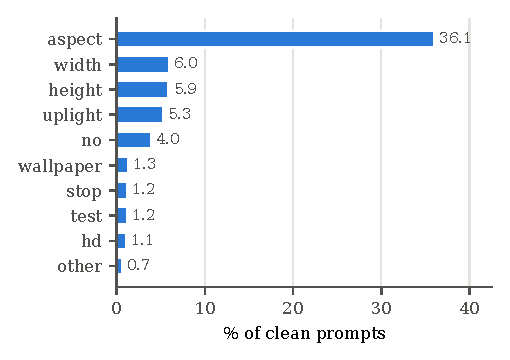
\includegraphics[width=\columnwidth]{figures/params}
\caption{Share of clean prompts using each parameter.}
\label{fig:params}
\end{figure}

\subsection{RQ2: Artists and Quality Boosters}
The share of prompts naming an artist is \PctArtistStrict\% under the
strict rule and \PctArtistLenient\% under the lenient rule: the rule alone
changes the answer by a factor of \ArtistRuleRatio. The most-cited names are concept and
fantasy illustrators such as \TopArtistOne{} and \TopArtistTwo{}
(Fig.~\ref{fig:artists}). \PctBoosterAny\% of prompts use at least one
booster phrase, most often ``\TopBoosterOne'', ``\TopBoosterTwo'' and
``\TopBoosterThree''.
% figures/boosters.pdf left out to save space; the text gives the top three.

\begin{figure}[t]
\centering
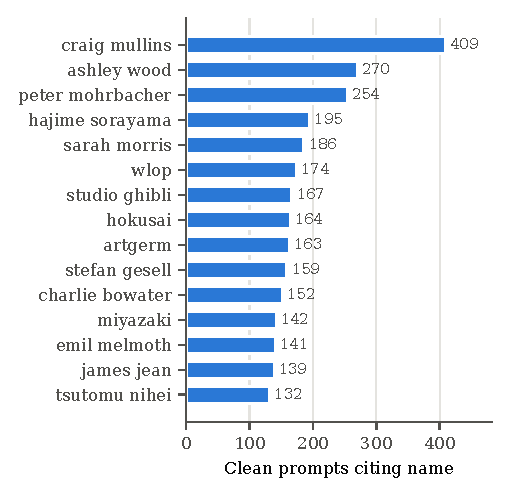
\includegraphics[width=\columnwidth]{figures/artists}
\caption{Most-cited artist or studio names (lenient rule).}
\label{fig:artists}
\end{figure}

\subsection{RQ3: Topics}
Table~\ref{tab:topics} lists the ten NMF topics. They separate rendering
style (octane/unreal render, oil painting, black-and-white ink,
hyper-realistic photo, vector art) more than subject matter, which is
consistent with booster phrases dominating word frequencies. Mean
stability across subsamples is $J=\TopicJaccard$; most topics are stable
($J>0.7$), but the least stable topic, a mix of artists' first names, is not
($J=\MinTopicJaccard$).
% Re-check these topic descriptions if k or the vocabulary rules change.

\begin{table}[t]
\centering
\caption{NMF topics: share of prompts, stability $J$, top words.}
\label{tab:topics}
\small
\begin{tabular}{rrrp{0.55\columnwidth}}
\toprule
\# & \% & $J$ & Top words \\
\midrule
1 & 7.8 & 0.80 & render, octane, unreal, engine, high, artstation \\
2 & 10.8 & 0.73 & style, ghibli, anime, poster, design, city \\
3 & 1.0 & 0.52 & artwork, van, john, peter, mike, robert \\
4 & 8.6 & 0.93 & art, concept, fantasy, circa, pulp, magazine \\
5 & 9.4 & 0.84 & painting, oil, matte, abstract, space, beautiful \\
6 & 19.2 & 0.93 & black, white, background, red, ink, photo \\
7 & 12.5 & 0.85 & portrait, beautiful, artstation, character, face, girl \\
8 & 9.9 & 0.79 & realistic, hyper, photo, ultra, old, epic \\
9 & 16.6 & 0.72 & detailed, cinematic, highly, lighting, intricate, dark \\
10 & 3.2 & 1.00 & vector, psychedelic, flat, rule, symmetrical, thirds \\
\bottomrule
\end{tabular}

\end{table}

\subsection{RQ4: Hypothesis Tests}
Prompts using a parameter are longer (median \MedianWordsParam{} vs.\ \MedianWordsNoParam{} content words;
Mann--Whitney $p<.001$, $r_{rb}=\HOneRankBiserial$, a medium effect).
Artist references and booster phrases are associated ($\chi^2(1)=\HTwoChi$,
$p<.001$), but the effect is negligible ($V=\HTwoCramersV$): \PctBoostIfArtist\% of
prompts naming an artist use a booster, against \PctBoostIfNoArtist\% of those
that do not.

\subsection{AI Tool Results}
\textit{Run A (Copilot).} Unprompted (P0), the tool led with data quality:
73.5\% of rows repeat an earlier row and 83.1\% of test rows occur in train,
so ``the existing splits [are] unreliable for measuring generalization''.
Its duplicate count matched the pipeline's exactly (180,983). In P1 it flagged a row
as ``not a real prompt'' only if the whole row was an aspect ratio, number,
parameters or URL (25.5\% of rows), noting that 52,970 rows of at most one
word were left in; the pipeline's three-word rule excludes \PctNonPrompt\%. This left
64,907 distinct rows, 13\% more than the pipeline's. Its median length matches the pipeline's (12), but it counted whitespace items including parameter flags, and 7.9\%
of its rows were a single item; these short rows rarely carry parameters,
which lowers its parameter shares. The top aspect ratios agree (16:9, 9:16,
2:3). For artists (P3) it mined names after cues such as ``in the style
of'' and then searched a fixed list of 50; the mining output was not kept,
so the list cannot be traced to a rule. It found 13.5\%, just below the pipeline's strict rule (\PctArtistStrict\%),
with the same top name (\TopArtistOne). Its six booster phrases
(three from the prompt, three its own) found 21.8\%. For topics (P4) it chose the pipeline's method and settings (TF-IDF, NMF, $k=10$) and
found nearly the same topics, down to a 0.9\% topic of artists' first names; two reruns gave
matched cosine similarity 0.88 and 0.76, which it called ``not highly
stable''. For H1 (P5) it reported $r_{rb}=0.60$, and noted that its length
measure counts the parameters themselves (0.49 without them). For H2 it
reported an odds ratio of 2.84 (39.9\% vs.\ 18.9\% booster use) and
$p\approx1.7\times10^{-3677}$, a spuriously precise figure. It called both
results ``associations, not causal findings''. Its P6 code was ``a
consolidated, verified reproduction, not a verbatim transcript''; run with the pipeline's library versions, it reproduced every number in
P1--P5.

\textit{Run B (Claude).} Run B matched run A's exact counts but chose definitions much closer to the pipeline's, and so did its numbers
(Table~\ref{tab:compare}). It treated a row as a fragment only if it was a
single word, supported by showing that 96.7\% of such rows occur inside
longer prompts, which left 59,733 prompts (4\% more than the pipeline's). It removed
parameters before counting words, so its median and H1 effect
($r_{rb}=0.41$) almost match the pipeline's. For artists it combined a wording rule
(17.2\%) with 168 names mined from the data (21.3\%), checking ambiguous
names by hand (e.g.\ excluding ``M\"obius strip''). For topics it chose $k$
by coherence and stability, fitted a second model without style words, and
compared NMF with LDA (top-word overlap 0.17--0.23), concluding that topic
shares ``can move by tens of points between runs''. On H2 it found the same
raw association as run A (OR $=2.17$) but then controlled for prompt
length, since artist prompts are longer: the odds ratio fell to 0.95
(logistic regression) and 1.01 (Mantel--Haenszel). It also claimed the data
show a content filter, which the data alone cannot establish. The tool reports that its rewritten P6 code reproduced every number; this
has not yet been checked by re-running it. \todo{If run A's tool is run again, report the spread across
runs.}

%%%%%%%%%%%%%%%%%%%%%%%%%%%%%%%%%%%%%%%%%%%%%%%%%%%%%%%%%%%%%%%%%%%%%%%%%%%%%%
\section{Discussion}
%%%%%%%%%%%%%%%%%%%%%%%%%%%%%%%%%%%%%%%%%%%%%%%%%%%%%%%%%%%%%%%%%%%%%%%%%%%%%%

\subsection{Interpretation}
The two analyses agree wherever the question has one obvious answer:
exact duplicates, train--test leakage, the most common aspect ratios and
artists, and, given the same model settings, the topics. They differ
wherever the analyst must define a variable, and every difference in
Table~\ref{tab:compare} traces to one of four decisions: (1)~the
\emph{non-prompt rule}, where run A kept short fragments that lower its
parameter shares; (2)~the \emph{length unit}, where counting parameter
tokens as words inflates the H1 effect from \HOneRankBiserial{} to 0.60;
(3)~the \emph{artist rule}; and (4)~the \emph{booster list}. Decisions (3)
and (4) together change the H2 conclusion. The scripted pipeline finds the association negligible ($V=\HTwoCramersV$, a 9-point gap); run A's figures (OR $2.84$,
a 21-point gap) would usually be read as a real, small-to-moderate effect;
run B adds a third reading, that the association almost vanishes once
prompt length is controlled. None of these is wrong; each answers a
differently defined question. This is the ``many analysts'' result
\cite{silberzahnManyAnalysts2018} with AI tools as two of the analysts.

On rigor, both tools did better than expected: they found the data
problems unasked, reported effect sizes, ran sensitivity checks and stated
the limits of their rules. Their weaknesses lay in what they left unseen:
exploratory steps that shaped the artist lists, and final code rewritten
after the fact. Run A also made one numerical error, which it caught
itself in P6.

\subsection{Validity}
\textit{Construct validity.} ``Names an artist'' and ``uses a booster''
depend on the rule. The strict and lenient rules differ by a factor of
\ArtistRuleRatio, and the tool's list gives a third answer. To estimate how
well the rules work, each author labelled the same random sample of 100
clean prompts on their own. \todo{Report precision and recall of each rule
against the agreed labels, and Cohen's $\kappa$ between the two raters,
from section 7 of explore.ipynb.} \textit{Internal validity.} RQ4 tests
associations only; prompts were not assigned to conditions, and
near-duplicate templates break the independence the tests assume, so the
$p$-values are too small. \textit{External validity.} The data come from
one Discord community in 2022, mostly in English, using early Midjourney
versions. They do not describe prompting today or on other tools.

\subsection{Ethics}
The Discord users who wrote these prompts did not consent to research use.
The dataset drops user names, but prompts can still contain personal names
or identifying text, so only aggregates are reported and no prompt that names a private
person is quoted. Many prompts ask for the style of living artists,
which is the centre of an open dispute over consent and copyright; this study counts these names but does not judge the practice. Some prompts may be
sexual or violent; they were not filtered, but the examples in this paper avoid them.
The Apache-2.0 licence was applied to scraped third-party text, so it may
not settle the authors' rights. Run A raised none of these issues, even
when asked open-ended questions; run B raised only the copyright point,
noting that many named artists are living illustrators.

\subsection{Reproducibility and AI Transparency}
Re-running the scripted pipeline rebuilds every number in this paper
(Appendix~\ref{app:repro}). The AI arm is harder to repeat. Run A's model
is known only by an internal name and may change without notice, and
settings such as memory were recorded by the operator, not the tool. Both
tools' working steps, including the output that shaped the artist lists,
were not kept, and their final code was a rewrite of what they ran; run A's
rewrite gave the same numbers, but a rewrite could hide a step that
mattered. Run B also used newer libraries (Python 3.15, scikit-learn 1.9.1),
so its topic figures may not repeat exactly. Since the runs used different
tools, they show how much two AI analysts disagree, not how much one tool
varies between runs. In the authors' setup, a Windows checkout let Git convert
the CSV's line endings, breaking its SHA-256 check; a \texttt{.gitattributes}
rule now stores data files byte-for-byte. To repeat the AI analysis a reader
needs the tool, model, date, settings, input hash, exact prompts
(Appendix~\ref{app:prompts}) and full logs, all of which are supplied; even then, the
answers may differ.

%%%%%%%%%%%%%%%%%%%%%%%%%%%%%%%%%%%%%%%%%%%%%%%%%%%%%%%%%%%%%%%%%%%%%%%%%%%%%%
\section{Conclusion}
%%%%%%%%%%%%%%%%%%%%%%%%%%%%%%%%%%%%%%%%%%%%%%%%%%%%%%%%%%%%%%%%%%%%%%%%%%%%%%

Fewer than half the rows in this widely used prompt dataset are prompts,
three in four repeat an earlier row, and most test rows also appear in
training, so it must be cleaned and re-split before use. Given the same data
and questions, the AI tools matched the scripted pipeline on every quantity with one
obvious definition and diverged on every quantity that needed a judgement,
in one case enough to change the conclusion. Anyone using an AI tool for analysis should ask it to state each
definition before it computes anything, keep the full log, and re-run the
analysis with independent code before reporting it.

%%%%%%%%%%%%%%%%%%%%%%%%%%%%%%%%%%%%%%%%%%%%%%%%%%%%%%%%%%%%%%%%%%%%%%%%%%%%%%
\section*{Use of AI Tools}
%%%%%%%%%%%%%%%%%%%%%%%%%%%%%%%%%%%%%%%%%%%%%%%%%%%%%%%%%%%%%%%%%%%%%%%%%%%%%%

The AI-assisted analysis (Part~1a) used the two tools described in
Section~III-C; the prompts are in Appendix~\ref{app:prompts} and the full
logs are supplementary files. The scripted pipeline (Part~1b) and the first draft of this paper's structure
were written with help from Claude Opus~5.5 (Anthropic), through Claude
Code. Claude also scored run~A against the pipeline's results, re-ran the tool's code,
and drafted the AI results, Discussion and Conclusion from the run logs. The authors reviewed and ran all code, checked every reported number against the
pipeline output and the logs, and are responsible for the final content.

\bibliographystyle{IEEEtran}
\bibliography{a3references}

\appendices

\section{Prompts Given to the AI Tool}
\label{app:prompts}
Each prompt was pasted exactly as below, in order, in one new chat. If the
tool had stopped, the only allowed reply was ``Please continue.'' The full
run logs, the tool's code and the scoring sheet are supplied as
supplementary files (\texttt{ai-analysis/runs/}).

\textbf{P0.} I have uploaded a dataset of text-to-image prompts collected
from the Midjourney Discord server. Analyse this dataset and report your
main findings.

\textbf{P1.} How clean is this dataset? Report how many rows are empty,
duplicated, or are not real prompts, and whether rows in the validation
and test splits also appear in the train split. Explain exactly how you
decided what counts as ``not a real prompt''.

\textbf{P2.} Excluding rows that are not real prompts and removing
duplicates, describe what a typical prompt looks like: its length in
words, how often Midjourney parameters such as \texttt{--ar},
\texttt{--no}, \texttt{--w}/\texttt{--h}, \texttt{--stop} and
\texttt{--seed} are used, and the most common aspect ratios.

\textbf{P3.} What share of prompts reference a named artist or ``in the
style of'' someone? Which artists are named most often? What share use
generic quality phrases such as ``trending on artstation'', ``8k'' or
``octane render''? State the rule you used to detect each.

\textbf{P4.} Identify the main themes or topics in the prompts using a
topic model. Report the topics with their top words and the share of
prompts in each. How stable are these topics if the analysis is re-run?

\textbf{P5.} Test two hypotheses and report the test, test statistic,
p-value and an effect size for each: (H1) prompts that use at least one
parameter are longer than prompts that use none; (H2) prompts that name
an artist are more likely to use a quality phrase.

\textbf{P6.} Give me the complete code you ran for all of the above, in
one block, so that I can reproduce your results.

\section{Reproducibility Details}
\label{app:repro}
\textit{Data.} \texttt{succinctly/midjourney-prompts}, Parquet files
downloaded from Hugging Face on 6 Nov.\ 2026. SHA-256:
train \texttt{c13d7d1e\ldots0a62b},
validation \texttt{553a0a02\ldots9c5539},
test \texttt{57f8a944\ldots490eb0}.
The combined CSV given to the AI tool has SHA-256
\texttt{582e6d09\ldots934806} with LF line endings.

\textit{Environment.} Python 3.8.10, NumPy 1.24.4, pandas 2.0.3,
SciPy 1.10.1, scikit-learn 1.3.2, Matplotlib 3.7.5, PyArrow 14.0.2;
random seed 9200.

\textit{Commands.} \texttt{python3 analysis/fetch\_data.py} downloads and
checks the files; \texttt{python3 analysis/pipeline.py} writes every
number, table and figure; \texttt{latexmk -pdf} builds this paper.

\end{document}
